%% Добавить иллюстрацию 1 - images/1.jpg (jpg -> tikz)
% \begin{figure} 
%     \centering
%     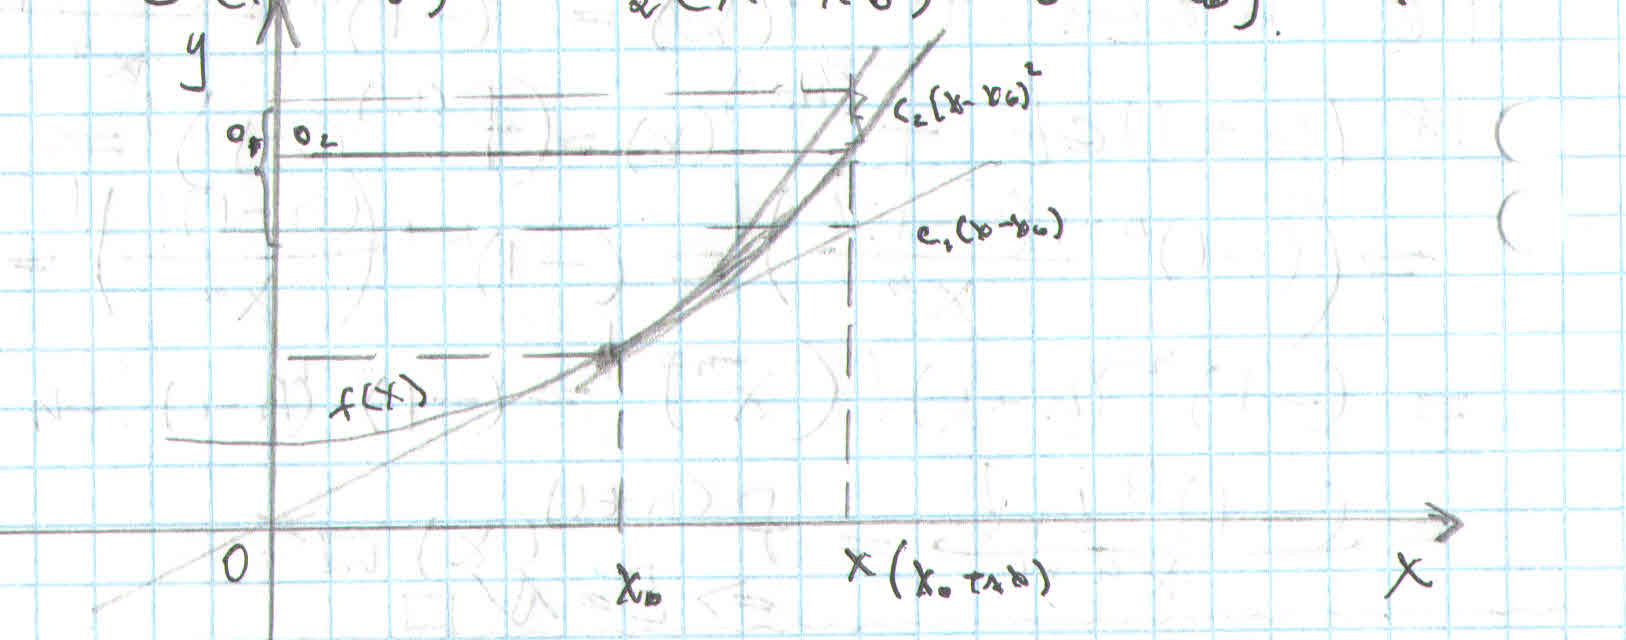
\includegraphics[width=0.5\textwidth]{1}
%     \caption{\label{fig:diffGeom} Приближение при помощи дифференциалов}
% \end{figure}
\begin{figure} 
    \centering
    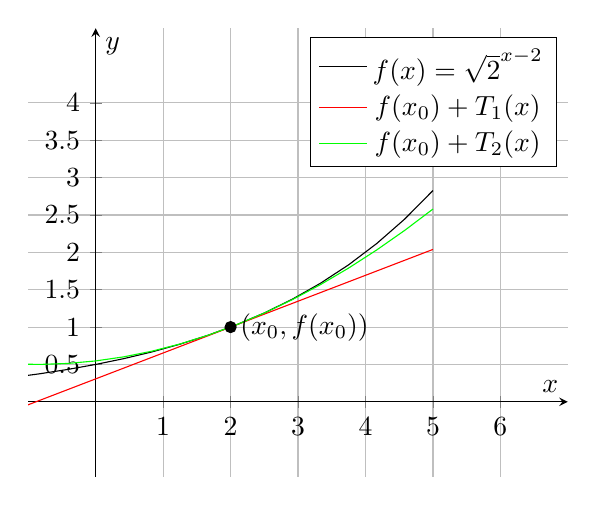
\begin{tikzpicture} 
        \begin{axis} [
            xmin = -1, xmax = 7,
            ymin = -1, ymax = 5,
            grid=major,
            axis lines = middle,
            xlabel=\( x \),
            ylabel=\( y \),
            xtick={0, 1, 2, ..., 6},
            ytick={0, 0.5, 1, ..., 4}
        ]
            \legend{
                \( f(x) = \sqrt{2}^{x-2} \),
                \( f(x_0)+T_1(x) \),
                \( f(x_0)+T_2(x) \)
            }
            \addplot[black] {(sqrt(2))^(x-2)};
            \addplot[red] {1 + ln(sqrt(2))*(x-2)};
            \addplot[green] {1+ln(sqrt(2))*(x-2)+(((ln(sqrt(2)))^2)/2)*((x-2)^2)};
            \addplot[only marks, mark=*] coordinates{(2, 1)} node [right] {\( (x_0, f(x_0)) \)};
        \end{axis}
    \end{tikzpicture}
    \caption{\label{fig:diffGeom} Приближение при помощи дифференциалов}
\end{figure}